\Chapter{Szuperpixel}

Miután a K-means módszer segítségével nem sikerült megfelelően megvalósítanom a szegmentálást, így más megközelítést kerestem. Számos tudományos cikkben láttam említést az úgynevezett szuperpixelekről, így végül erre a módszerre esett a választásom.

A szuperpixel módszer során a pixelekből nagyobb csoportokat, úgynevezett szuperpixeleket képez az algoritmus. A pixelek csoportosításához különféle jellemzők állnak rendelkezésre, például a fényerő, az intenzitás, a textúra, a kontúr. A szuperpixeleket számos területen használják, mint a képszegmentálás, a csontvázolás (skeletonization), az objektum lokalizálás, és a képindexelés. Maguk a szuperpixelek a túlzott szegmentálás eredményei.

Általánosságban elmondható, hogy a szuperpixel módszereknek 2 csoportja van, a gradiens-emelkedésen (gradient-ascent) alapuló algoritmusok, és a gráf-alapú algoritmusok.

A gráf-alapú algoritmus minden egyes képpontot egy gráf csomópontjaként kezel, és a két csomópont közötti élsúlyokat a képpontok közötti hasonlósággal arányosan határozza meg. Az egyik módszer amit teszteltem, a Felzenszwalb algoritmus egy példa a gráf-alapú algoritmusokra.

A gradiens-emelkedés alapú algoritmusok durva klaszterezéssel kezdenek. Ez egy iteratív folyamat, ahol minden egyes iteráció során az előző iterációból új klasztereket finomítanak a jobb szegmentáció elérése érdekében, amíg a konvergenciát el nem érik. A másik három módszer amit teszteltem, a SLIC, a Quick shift és a Watershed ebbe az osztályba tartozik. \cite{superpixel}

A következő fejezetekben röviden ismertetem a módszereket. A \texttt{skimage} könyvtárban megtalálható \texttt{felzenszwalb}, \texttt{slic}, \texttt{quickshift}, és \texttt{watershed} algoritmusokat használtam a vizsgálatok során.

\Section{Felzenszwalbs módszer}

Ez az algoritmus népszerű számítógépes látás területén. Egy fontos paraméterrel rendelkezik, ami a \texttt{scale}, ez befolyásolja a szegmensek méretét. A szegmensek száma és tényleges mérete jelentősen változhat a képek helyi kontrasztjától függően. Ez az algoritmus mind valós, mind szintetikus képek szegmentálását biztosítja, és széles körben inkább szegmentáló algoritmusként, mint szuperpixel algoritmusként ismert.

Általában a gráf alapú algoritmusok bemenete egy $G \frac{1}{4} (V, E)$ gráf, $n$ csúccsal és $m$ éllel. A kimenet $V$-nek a szegmentálása $S \frac{1}{4} (C_1, C_2, \dots, C_r)$ komponensekre. A szegmentáláshoz Dijkstra algoritmusát szokták használni.\cite{superpixel} \cite{superpixel_example}

A módszert a következő kódrészletben található módon használom.
\begin{python}
from skimage.segmentation import felzenszwalb

segments_fz = felzenszwalb(image, scale=100, sigma=0.5, min_size=50)
\end{python}

\Section{SLIC módszer}

A SLIC K-means klaszterezést használ a szuperpixelek létrehozásához méghozzá az 5D térben, amely a pixelek helyzete mellett a színekről is tartalmaz információt. Alapértelmezés szerint az egyetlen szükséges paraméter a K, ami a szuperpixelek számának beállítására szolgál, vagyis ennek segítségével tetszés szerint tudjuk szabályozni a szuperpixelek méretét. A SLIC színes és szürkeárnyalatos képekre egyaránt használható, ehhez a \texttt{compactness} értéket kell színes képek esetén magasabb, szürkeárnyalatos képek esetén alacsonyabb értékre beállítani, hiszen ezzel adjuk meg azt, hogy az algoritmus mekkora hangsúlyt fektessen a színekre a képen.

A SLIC algoritmus három fő lépésre oszlik hasonlóan a K-means algoritmushoz. Az első az inicializálási lépés, amelyben a klaszterek inicializálása történik. A második hozzárendelési lépésben minden egyes pixel a legközelebbi klaszterközépponthoz társul, ha a keresési régió átfedésben van a helyével. Végül a harmadik lépésben a klaszterközéppontok frissülnek, hogy a klaszterhez tartozó összes pixel átlagvektorává váljanak.

 A már említett \texttt{compactness} paraméter mellett fontos paraméter még a K értékét, vagyis a szegmensek számát megadó \texttt{n\_segments}. \cite{superpixel} \cite{superpixel_example}

A módszert a következő kódrészletben található módon használom.
\begin{python}
from skimage.segmentation import slic

segments_slic = slic(
    resized_image,
    n_segments=250,
    compactness=.1,
    sigma=5,
    start_label=0)
\end{python}

\Section{Quick shift módszer}

A Quick shift egy viszonylag új keletű 2D-s képszegmentáló algoritmus, amely a kernelizált átlageltolás közelítésén alapszik. A helyi módkereső algoritmusok családjába tartozik és Parzen sűrűségbecslést használ.

Ha van egy $N$ hosszúságú bemenetünk, amelynek az alakja $x_1, x_2, \dots, x_N \in X = R^d$, akkor az algoritmus a Parzen sűrűségbecsléssel kezdődik aminek a képlete a következő:

\[ P(x) =\frac{1}{N} \sum_{i=1}^{N} k(x-x_i), \quad x \in R^d \]

Ezt a módszert is, hasonlóan a SLIC módszerhez az 5D térben alkalmazzák, amely a pixelek helyzete mellett a színekről is tartalmaz információt.

A Quick shiftnek két fő paramétere van: a \texttt{sigma}, ami a helyi sűrűség közelítés skáláját vezérli, és a \texttt{max\_dist}, ami pedig kiválaszt egy szintet az előállított hierarchikus szegmentációban. Fontos paraméter még a \texttt{ratio}, amely kompromisszum a szín fontossága és a térbeli fontosság között. \cite{superpixel} \cite{superpixel_example}

A módszert a következő kódrészletben található módon használom.
\begin{python}
import cv2
from skimage.segmentation import quickshift

grayscaled_color = cv2.cvtColor(resized_image, cv2.COLOR_GRAY2RGB)

segments_quick = quickshift(
    grayscaled_color,
    kernel_size=3,
    max_dist=6,
    ratio=0.5)
\end{python}

\Section{Watershed módszer}

Ez a módszer intelligens módon használja a watershed transzformációt és a topológiai gradiens megközelítést. Ahelyett, hogy színes képet fogadna el bemenetként, szürkeárnyalatos gradiens képet vesz, ahol a világos pixelek a szegmensek vagy régiók közötti határokat jelölik.

A szürkeárnyalatos képeket topográfiai domborzatnak tekinti, és minden egyes domborzatot eláraszt a minimumától. Egy gát akkor épül, ha két tó összefolyik, az összes gát halmaza határozza meg az úgynevezett vízgyűjtőt. A vízgyűjtők ilyen ábrázolása a természetes áradási folyamatot szimulálja. A bemeneti képet tájképnek veszi, ahol a világos pixelek magas csúcsokat alkotnak. Minden egyes vízgyűjtő végül egy egyedi szegmenst alkot.

A SLIC-hez hasonlóan van egy \texttt{compactness} paramétere, amely megnehezíti a markerek számára a távoli képpontok elárasztását. Ez szabályosabbá teszi a vízválasztó régiókat. \cite{superpixel} \cite{superpixel_example}

A módszert a következő kódrészletben található módon használom.
\begin{python}
from skimage.segmentation import watershed
from skimage.filters import sobel

gradient = sobel(image)

segments_watershed = watershed(gradient, markers=250, compactness=0.001)
\end{python}

\Section{Összegzés}

Az említett módszerek teszt futását a \ref{fig:superpixel_example}. ábra tartalmazza.

\begin{figure}[h]
\centering
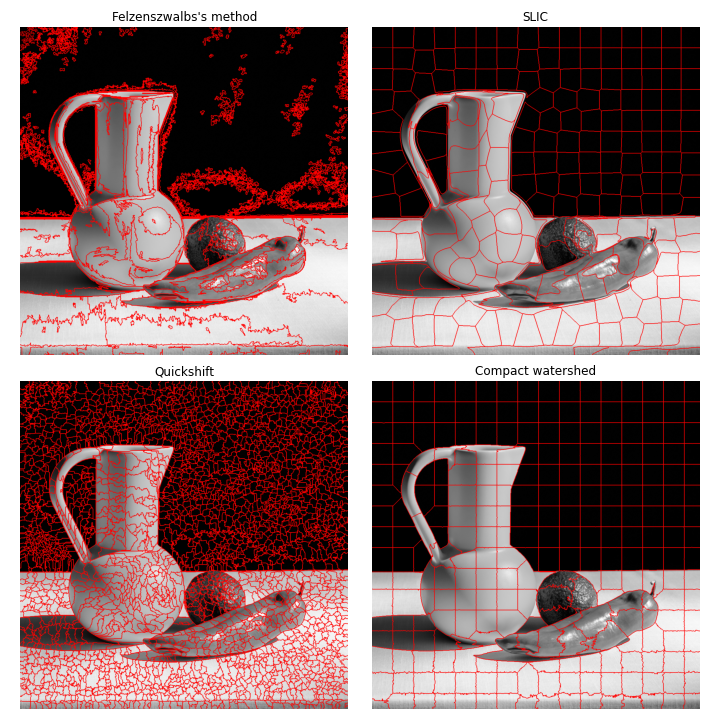
\includegraphics[scale=0.6]{images/superpixel_example.png}
\caption{Példa a szuperpixel algoritmusok futására. }
\label{fig:superpixel_example}
\end{figure}

Jól látható, hogy a legjobb eredményt a SLIC és a Watershed algoritmusok eredményezték. Ezen algoritmusok esetében szépen elkülönülnek egymástól az objektumok, és kevésbé befolyásolja az eredményt a tárgyakon megtalálható árnyék nem úgy, mint a K-means esetében.

Mivel a SLIC és a Watershed bizonyult a 4 módszer közül a legjobbnak, így ezeket fogom használni a színezési vizsgálatok során.
